\documentclass[a4paper, 11pt]{article}

% packages
\usepackage[utf8]{inputenc}
\usepackage{amsmath}
\usepackage{amsfonts}
\usepackage{array}
\usepackage{booktabs}
\usepackage{chngcntr}
\usepackage{colortbl}
\usepackage{dcolumn}
\usepackage{floatrow}
\usepackage{geometry}
\usepackage{graphicx}
\usepackage{hyperref}
\usepackage{multirow}
\usepackage{natbib}
\usepackage[normalem]{ulem}
\usepackage{ntheorem}
\usepackage{pdflscape}
\usepackage{rotating}
\usepackage{setspace}
\usepackage{subfigure}
\usepackage{tabularx}
\usepackage{threeparttable}
\usepackage[numbib, nottoc, notlot, notlof]{tocbibind}
\usepackage{wrapfig}
\usepackage{xcolor}

% page styling
\geometry{
  a4paper,
  left=1in,
  right=1in,
  bottom=1.2in,
  top=1.2in
}
\pagestyle{plain}
\pagenumbering{arabic}
\linespread{1.5}
\hypersetup{
  colorlinks,
  linkcolor={red!50!black},
  citecolor={blue!50!black},
  urlcolor={blue!80!black}
}
\theoremseparator{:}
\newtheorem{hyp}{Hypothesis}
\counterwithin*{hyp}{section}

\renewcommand{\thefootnote}{\fnsymbol{footnote}}

\title{
	Party Nomination Strategy and its Representational Consequences in Interactive Mixed-Member Majoritarian Systems
	\footnotemark{}
	\footnotetext[1]{This paper was previously entitled and circulated as ``Youth Underrepresentation and Parties' Nomination Strategy in Mixed-Member Electoral Systems". Earlier versions of this paper were presented at the 2024 summer meeting of the Japanese Society for Quantitative Political Science (JSQPS) and 2024 Annual Meeting of Americal Political Science Association (APSA). I thank Dan Smith for sharing the latest version of his data, and Serika Atsumi, Yuki Atsusaka, Amy Catalinac, Kentaro Fukumoto, Yusaku Horiuchi, Junko Kato, Kenneth McElwain, Mayuko Toba, Masahiro Yamada, Hironao Yoda for their comments.}
}

\author{
	Dai Sasaki
	\thanks{Master's Student, Graduate Schools for Law and Politics, The University of Tokyo. Email: daichansama12@g.ecc.u-tokyo.ac.jp; Website: https://dxxsxsxkx.github.io.}
}

\date{
	First Version: 28 Jun, 2024 \\
	This Version: 6 Dec, 2024 
}

\begin{document}

\maketitle

\renewcommand{\thefootnote}{\arabic{footnote}}
\setcounter{footnote}{0}

\begin{abstract} 
I argue that interactive mixed-member majoritarian systems (interactive MMMs), a variant of mixed member systems where parties can nominate the same candidates in both majoritarian and proportional representation (PR) tiers (dual listing), diminish the representational advantages commonly associated with PR systems. Analyzing comprehensive, candidate-level data of Japan's lower house elections, I show that parties give higher list ranks to senior candidates, incumbents, and dual-listed candidates. Furthermore, incumbents are more likely to be dual-listed than non-incumbents. These patterns apply across parties, but are less applicable to situations of intra-party disputes and government transitions, where seniors and incumbents may give their way to newcomers. My analysis suggests that interactive MMMs sustain representational inequalities between groups by reducing the electoral prospects of newcomers and making legislative turnover less frequent.
\end{abstract}

\newpage

\section{Introduction}

% TODO: write

\section{Theory} \label{sec: the}

\subsection{Theoretical Expectations}

% TODO: write

\subsection{Case: Japan's Mixed-Member Majoritarian System}

% TODO: write

\section{Data and Method} \label{sec: emp}

% TODO: write

\section{Result} \label{sec: res}

\subsection{Aggregate-Level Analysis}

% TODO: write

\subsection{Party-Specific Analysis}

% TODO: write

\subsection{Election- / Party-Specific Analysis}

% TODO: write

\section{Discussion} \label{sec: dis}

% TODO: write

\subsection{Legislative Turnover}

% TODO: write

\subsection{Representation}

% TODO: write

\begin{table}[htbp]
\begin{center}
\begin{threeparttable}
% latex table generated in R 4.1.0 by xtable 1.8-4 package
% NOTE: manually modified on 27 Nov 2023. 
% Sat Jul  8 06:31:47 2023
\begin{tabular}{lccccc}
\toprule
Country & Eligibility & Average & \% U30 & \% U40 & \% U45 \\ 
\midrule
Canada & 18 & 50 & 1.95 & 16.88 & 30.19 \\ 
France & 18 & 49 & 4.85 & 26.52 & 37.95 \\ 
Germany & 18 & 47 & 8.83 & 28.94 & 41.98 \\ 
Italy & 25 & 49 & 1.25 & 16.25 & 35 \\ 
Japan & 25 & 55 & 0.22 & 6.02 & 17.2 \\ 
UK & 18 & 51 & 3.69 & 21.69 & 34 \\ 
USA & 25 & 57 & 0.46 & 10.42 & 20.14 \\ 
\bottomrule
\end{tabular}

\begin{tablenotes}[flushleft]
  \scriptsize{
    \item{\textit{Note.} Age demographics of lower house members in the G7 countries, as of January 2023. Eligibility is the minimum age to run for the house.}
    \item{\textit{Source.} \citet{inter-parliamentaryunionDataAgeCountry2024}.}
  }
\end{tablenotes}
\end{threeparttable}
\caption{Age Demographics of Lower Houses in the G7 Countries}
\label{table:intl}
\end{center}
\end{table}



\begin{figure}[!htbp]
	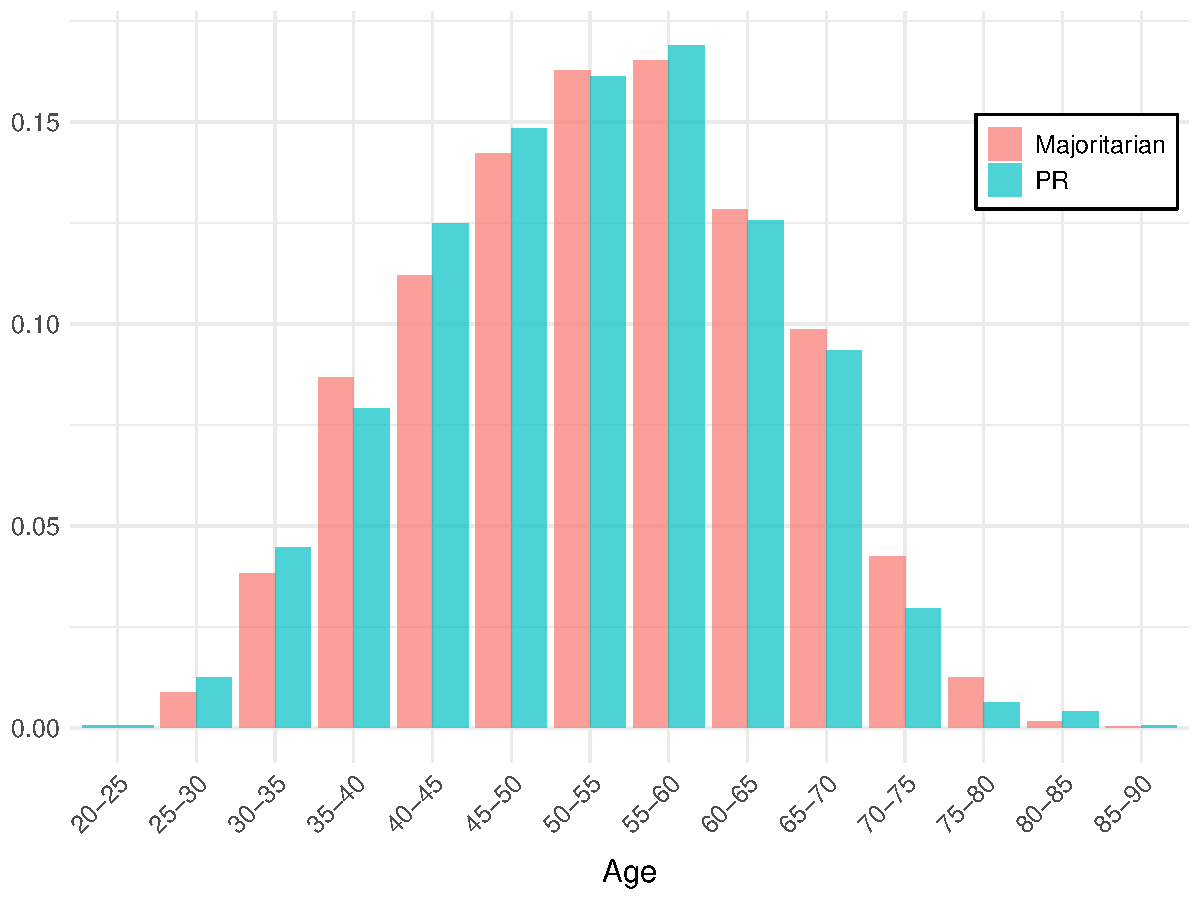
\includegraphics[width = 0.9\textwidth]{../figure/paper/age_smd_vs_pr_winners.pdf}
	\caption{Age Composition of Legislators Elected from the Two Tiers}
	\label{fig:pr_vs_smd}
\end{figure}



\begin{figure}[!htbp]
	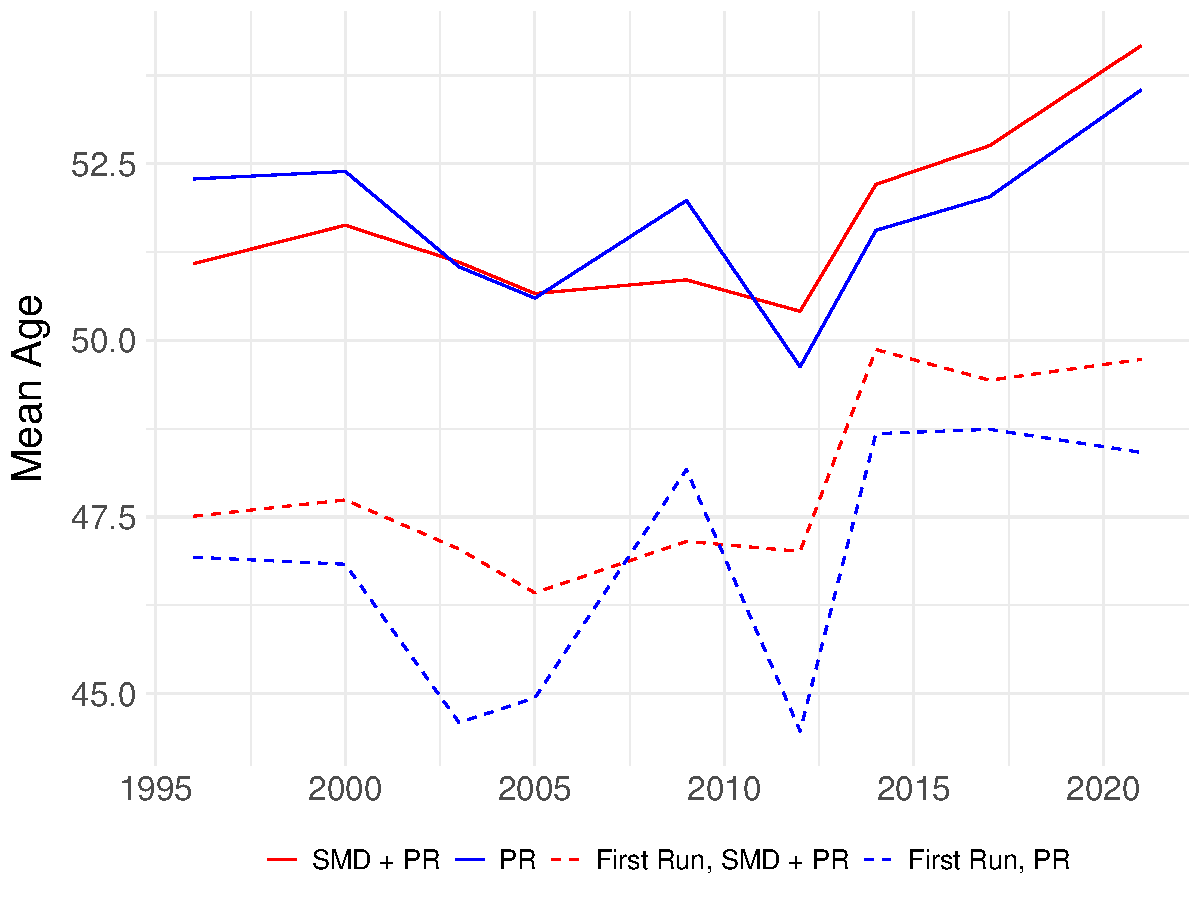
\includegraphics[width = 0.9\textwidth]{../figure/paper/age_first_run.pdf}
	\caption{Age Comparison: Average vs. New Candidates}
	\label{fig:ageFirstRun}
\end{figure}



\section{Conclusion}

% TODO: write

\newpage

\bibliography{../bibliography.bib}
\bibliographystyle{apalike}

\newpage

\appendix

\setcounter{table}{0}
\setcounter{figure}{0}
\renewcommand{\thetable}{A\arabic{table}}
\renewcommand{\thefigure}{A\arabic{figure}}

\section{Summary Statistics}

\subsection{Candidate-Level Summary}

% TODO: add a revised table

\newpage

\subsection{Magnitudes of PR Blocks, 1996 - 2017}

% created manually
\begin{table}[!htbp]
\begin{threeparttable}
\begin{tabular}{lccccccccc}
\toprule
Bloc & 1996 & 2000 & 2003 & 2005 & 2009 & 2012 & 2014 & 2017 & 2021 \\
\midrule
Hokkaido & 9 & 8 & 8 & 8 & 8 & 8 & 8 & 8 & 8 \\
Tohoku & 16 & 14 & 14 & 14 & 14 & 14 & 14 & 13 & 13 \\
Kita-kanto & 21 & 20 & 20 & 20 & 20 & 20 & 20 & 19 & 19 \\
Tokyo & 19 & 17 & 17 & 17 & 17 & 17 & 17 & 17 & 17 \\
Minami-kanto & 23 & 21 & 22 & 22 & 22 & 22 & 22 & 22 & 22 \\
Hokuriku Shinetsu & 13 & 11 & 11 & 11 & 11 & 11 & 11 & 11 & 11 \\
Tokai & 23 & 21 & 21 & 21 & 21 & 21 & 21 & 21 & 21 \\
Kinki & 33 & 30 & 30 & 30 & 29 & 29 & 29 & 28 & 28 \\
Chugoku & 13 & 11 & 11 & 11 & 11 & 11 & 11 & 11 & 11 \\
Shikoku & 7 & 6 & 6 & 6 & 6 & 6 & 6 & 6 & 6 \\
Kyushu & 23 & 21 & 21 & 21 & 21 & 21 & 21 & 20 & 20 \\
\bottomrule
\end{tabular}
\begin{tablenotes}[flushleft]
  \scriptsize{
    \item Magnitudes of each PR regional district for elections 1996 - 2021. 
    \item \textit{Data source}: \citet{reedReedSmithJapaneseHouse2017, ministryofinternalaffairsandcommunicationsElectionSenkyo2024}
  }
\end{tablenotes}
\end{threeparttable}
\caption{Magnitudes of PR Blocks}
\label{tab:distM}
\end{table}

\newpage

\subsection{Distribution of List Rank}

\begin{figure}[!htbp]
	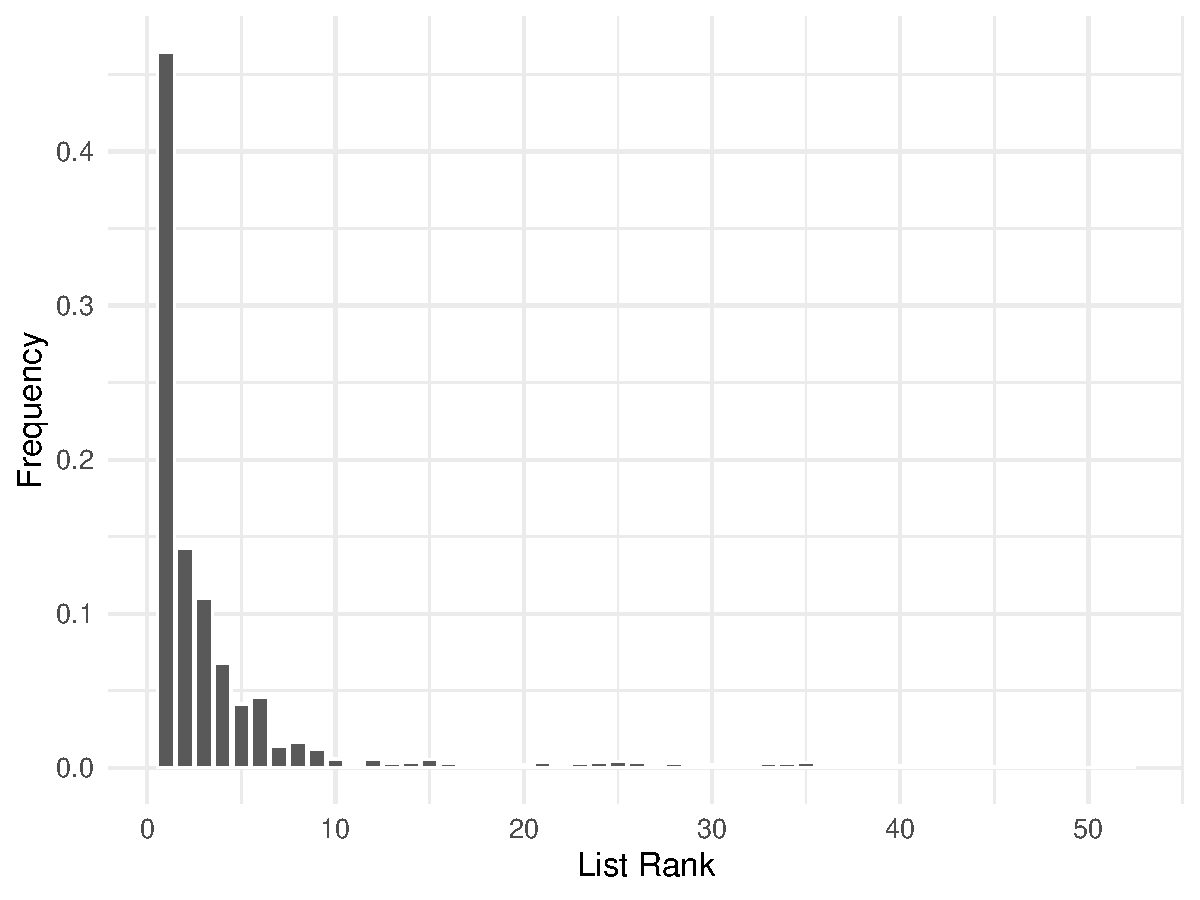
\includegraphics[width = 0.9\textwidth]{../figure/paper/pr_rank_distribution.pdf}
	\caption{Distribution of List Rank}
	\label{fig:distRank}
\end{figure}

\newpage

\subsection{Age of Winners}

\begin{figure}[!htbp]
	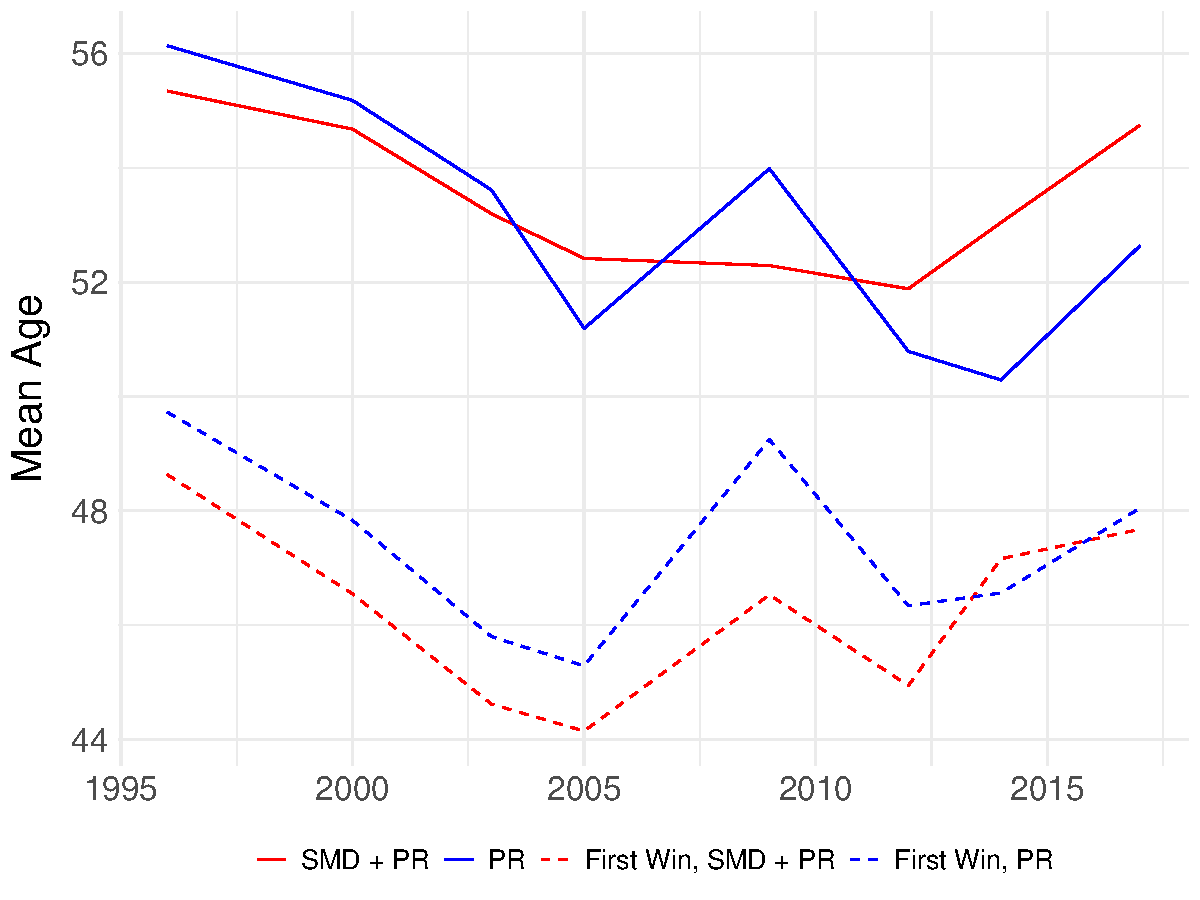
\includegraphics[width = 0.9\textwidth]{../figure/paper/age_first_win.pdf}
	\caption{Age Comparison: Average vs. New Legislators}
	\label{fig:ageFirstWin}
\end{figure}	

\end{document}































